\chapter{动量、能量守恒}
\section{作业习题}
\subsection*{一、填空题}
\begin{enumerate}
    \item 如图所示 \ref{fig:19} , 质量为$m$的子弹以水平速度$\vec{v_0}$射入静止的木块并陷入木块内, 
    设子弹入射过程中木块$M$不反弹, 则墙壁对木块的冲量$\vec{I}=\nl$ .
    \begin{figure}[H]
        \centering
        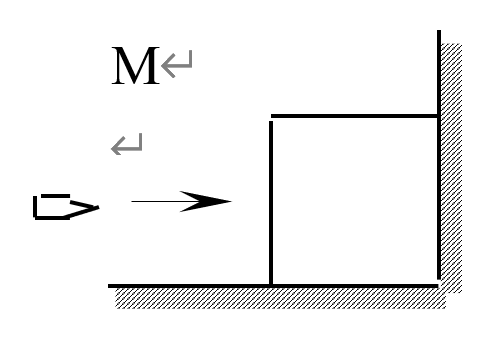
\includegraphics[width=0.15\textheight]{fig19}
            \caption{如图}\label{fig:19}
    \end{figure}
    \item 一质量为 $m$ 的物体, 以初速$\vec{v_0}$从地面竖直上抛, 如忽略空气阻力, 则从抛出到刚要接触地面的过程中,物体动量增量的大小为\nl .
    \item 一质量为$m$的物体作斜抛运动,初速率为$v_0$, 仰角为$\theta$. 如果忽略空气阻力, 物体从抛出点到最高点这一过程中所受合外力的冲量大小$I=\nl$.
    \item 有一质量为$M$的物体, 在光滑的水平面上沿直线滑行, 当它滑到某处速率为$v_0$时发生爆炸, 从主体上射出一质量为$m$的小块沿原方向水平飞行, 此时主体的速度为零, 则小块射出时对地的速率$v=\nl$.
    \item 一质量为$30 kg$的物体以$10m\cdot s^{-1}$的速率水平向东运动, 另一质量为$20 kg$的物体以$25 m\cdot s^{-1}$的速率水平向西运动. 两物体发生完全非弹性碰撞后, 它们的速度大小$v=\nl$.
    \item 质量为 $M$ 的平板车, 以速度$\vec{v}$在光滑的水平面上滑行, 一质量为$m$的物体从$h$高处竖直落到车子里,两者一起运动时的速度大小为$V=\nl$.
    \item 一颗质量为 $0.002kg$ , 速率为$700 m/s$的子弹, 打穿一块木板后,速率降到$400 m/s$, 则在此过程中受到的外力所做功$A=\nl$.
    \item 如图 \ref{fig:20} , 有人用恒力$F$, 通过轻绳和轻滑轮, 将一木块从位置$A$拉到位置$B$, 设物体原来位置$AC=L$, 后来位置$BC=L/2$, 物体水平位移为$S$, 则在此过程中,人所作的功为$A=\nl$.
    \begin{figure}[H]
        \centering
        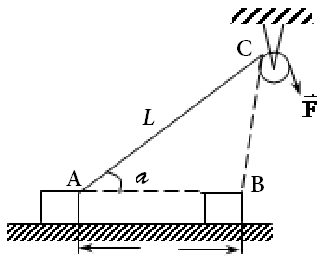
\includegraphics[width=0.15\textheight]{fig20}
            \caption{如图}\label{fig:20}
    \end{figure}
    \item 某质点在力$ \vec{F}=(5+5x)\vec{i}$ (SI)的作用下沿$x$轴作直线运动, 在从$x=0$移动到$x=20m$的过程中, 力$\vec{F}$所做的功为\nl .
    \item 如图所示\ref{fig:12} , 小球沿固定的光滑的$1/4$圆弧从$A$点由静止开始下滑, 圆弧半径为$R$, 则小球在$B$点处的法向加速度$a_n = \nl$; 切向加速度为 $a_t =\nl$. 
    \begin{figure}[H]
        \centering
        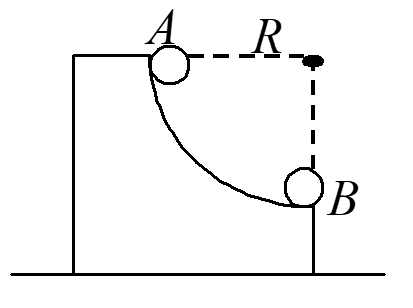
\includegraphics[width=0.15\textheight]{fig21}
            \caption{如图}\label{fig:21}
    \end{figure}
    \item 人造地球卫星, 质量为$m$, 在地球表面上空2倍于地球半径$R$的高度沿圆轨道运行, 卫星的万有引力势能为\nl. (用$m$、$R$、引力常数$G$和地球的质量$M$表示)
    \item 质量为$100kg$的货物, 平放在卡车底板上. 卡车以$5m/s^2$的加速度启动, 货物与卡车底板无相对滑动. 则在开始的4秒钟内摩擦力对该货物作的功$A=\nl$.
    \item 一个质量为$m=3kg$的质点, 在外力作用下, 运动方程为: $x=5+t^2$, $y=5t-t^2$, 则力在$t=0$到$t=2$秒内作的功为$A = \nl$.
\end{enumerate}
\subsection*{二、选择题}
\begin{enumerate}
    \item 一炮弹由于特殊原因在水平飞行过程中, 突然炸裂成两块, 其中一块作自由下落, 则另一块着地点(飞行过程中阻力不计):(\hspace{1pc})     
    \twoch{比原来更远;}{比原来更近;}{仍和原来一样远;}{条件不足,不能判定.}
    \item 质量为$0.02kg$的子弹, 以$400 m/s$的速率沿图示方向 \ref{fig:22} 射入一原来静止的质量为$0.98kg$的摆球中, 摆线长度不可伸缩. 子弹射入后开始与摆球一起运动的速率为(\hspace{1pc})
    \fourch{$2m/s$}{$4m/s$}{$7m/s$}{$8m/s$} 
    \begin{figure}[H]
        \centering
        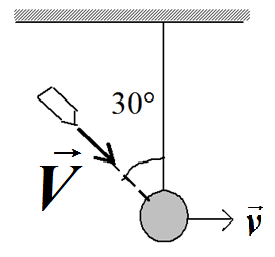
\includegraphics[width=0.15\textheight]{fig22}
            \caption{如图}\label{fig:22}
    \end{figure}
    \item 质量为$20 g$的子弹沿$x$轴正向以$500 m/s$的速率射入一木块后, 与木块一起仍沿$x$轴正向以$50 m/s$的速率前进, 在此过程中木块所受冲量的大小为(\hspace{1pc})                                                        
    \twoch{$9 N\cdot s$}{$11 N\cdot s$}{$10 N\cdot s$}{$-10 N\cdot s$}
    \item 质量为$m$的质点, 以不变速率$v$沿水平光滑轨道垂直撞击墙面, 撞击后被反弹, 假设撞击为完全弹性碰撞, 并规定碰撞前质点运动方向为正方向,则质点作用于墙面的冲量为(\hspace{1pc})
    \fourch{$mv$}{$2mv$}{$-mv$}{$-2mv$}

    \item 有两个完全相同的木块同时从同一高度自由落下, 在下落过程中有一水平方向飞来的子弹(其质量不可忽略不计)击中其中的一个木块, 并与木块一起下落, 则:(\hspace{1pc})  
   \twoch{两木块同时落地;}{被击中的木块后落地;}{被击中的木块先落地;}{无法判断}
   
   \item  两辆小车$A$、$B$, 可在光滑平直轨道上运动. $A$以$2 m/s$的速率向右与静止的$B$对心碰撞, $A$和$B$的质量相同, 假定车$A$的初始速度方向为正方向,则碰撞为完全弹性碰撞和完全非弹性碰撞时车$A$的速度分别为(\hspace{1pc})                         
   \twoch{$v_A=0 m/s$, $v_A=2 m/s$}{$v_A=0 m/s$, $v_A=1 m/s$}{$v_A=1 m/s$, $v_A=0 m/s$}{$v_A=2 m/s$, $v_A=1 m/s$}
    \item 一质量为$m$的质点, 自半径为$R$的光滑半球形碗口由静止下滑, 质点在碗内某处的速率为$v$, 则质点对该处的压力数值为(\hspace{1pc})                
    \fourch{$\frac{mv^2}{R}$}{$\frac{3mv^2}{2R}$}{$\frac{2mv^2}{R}$}{$\frac{5mv^2}{2R}$}
    \item 质量为$m=0.5kg$的质点, 在Oxy坐标平面内运动, 其运动方程为$x=5t$, $y=0.5t^2$(SI), 从$t=2s$到$t=4s$这段时间内, 外力对质点作的功为(\hspace{1pc})
    \fourch{$1.5 J$}{$4.5 J$}{$3 J$}{$-1.5 J$}

    \item 如图 \ref{fig:23} , 一质量为$m$的质点, 在半径为$R$的半球形容器中, 由静止开始自边缘上的$A$点滑下, 到达最低点$B$时, 它对容器的正压力为$N$. 则质点自$A$滑到$B$的过程中, 摩擦力对其作的功为(\hspace{1pc})
    \twoch{$\frac{1}{2}R(N-3mg)$}{$\frac{1}{2}R(3mg-N)$}{$\frac{1}{2}R(N-mg)$}{$\frac{1}{2}R(N-2mg)$}
    \begin{figure}[H]
        \centering
        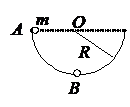
\includegraphics[width=0.15\textheight]{fig23}
            \caption{如图}\label{fig:23}
    \end{figure}
    \item 光滑水平面上有一质量为$m=1kg$的物体, 在力$\vec{F} = (1+x)\vec{i}$  (SI) 作用下由静止开始运动, 当物体从$x_1$处运动到$x_2$处, 在此过程中物体的动能增量为(\hspace{1pc})
    \twoch{$\left(x_1+\frac{x_1^2}{2}\right)-\left(x_2+\frac{x_2^2}{2}\right)$}{$\left(x_2+\frac{x_2^2}{2}\right)-\left(x_1+\frac{x_1^2}{2}\right)$}{$\left(x_1+\frac{x_1^2}{2}\right)$}{$\left(x_2+\frac{x_2^2}{2}\right)$}
    
    \item 在高台上分别沿$45^\circ$仰角方向和水平方向, 以同样速率投出两颗小石子, 忽略空气阻力, 则它们落地时速度(\hspace{1pc})
    \twoch{大小不同,方向不同;}{大小相同,方向不同;}{大小相同,方向相同;}{大小不同,方向相同.}
    \item 在经典力学中,关于动能、功、势能与参考系的关系,下列说法正确的是(\hspace{1pc})
    \onech{动能和势能与参考系的选取有关;}{动能和功与参考系的选取有关;}{势能和功与参考系的选取有关;}{动能、势能和功均与参考系选取无关.}
    \item 两辆小车$A$、$B$, 可在光滑平直轨道上运动. $A$以$3 m/s$的速率向右与静止的$B$碰撞, $A$和$B$的质量分别为$1kg$和$2kg$, 碰撞后$A$、$B$车的速度分别为$-1 m/s$和$2 m/s$, 则碰撞的性质为(\hspace{1pc})    
    \twoch{完全弹性碰撞;}{完全非弹性碰撞 ;}{非完全弹性碰撞 ;}{无法判断 .}
    \item $A$、$B$二弹簧的劲度系数分别为$k_A$和$k_B$, 其质量均忽略不计. 今将二弹簧连接起来并竖直悬挂, 如图所示\ref{fig:24} , 当系统静止时, 二弹簧的弹性势能$E_{PA}$与$E_{PB}$之比为(\hspace{1pc})                                                 
    \twoch{$\frac{E_{PA}}{E_{PB}}=\frac{k_B}{k_A}$}{$\frac{E_{PA}}{E_{PB}}=\frac{k_A^2}{k_B^2}$}{$\frac{E_{PA}}{E_{PB}}=\frac{k_A}{k_B}$}{$\frac{E_{PA}}{E_{PB}}=\frac{k_B^2}{k_A^2}$}
    \begin{figure}[H]
        \centering
        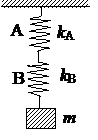
\includegraphics[width=0.15\textheight]{fig24}
            \caption{如图}\label{fig:24}
    \end{figure}
    \item 质点的动能定理: 外力对质点所做的功, 等于质点动能的增量, 其中所描述的外力为(\hspace{1pc})                                           
    \twoch{质点所受的任意一个外力;}{质点所受的保守力;}{质点所受的非保守力;}{质点所受的合外力.}
   
\end{enumerate}
\subsection*{三、计算题}
\begin{enumerate}
    \item 一个质量为$M$的四分之一圆弧形槽的大物体, 半径为$R$, 停在光滑的水平面上, 另一质量为$m$的物体, 自圆弧槽的顶端由静止下滑 (如图所示\ref{fig:25}) .
    求当小物体$m$滑到弧底时, 大物体在水平面上移动的距离为多少?
    \begin{figure}[H]
        \centering
        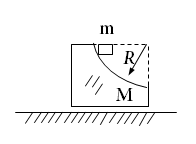
\includegraphics[width=0.15\textheight]{fig25}
            \caption{如图}\label{fig:25}
    \end{figure}
    \item 一个质量为$M=10kg$的物体放在光滑水平面上, 并与一水平轻弹簧相连, 如图\ref{fig:28}, 弹簧的劲度$K=1000N·m-1$, 今有一质量为$m=1kg$的小球, 
    以速度$V_0=4m\cdot s^{-1}$沿水平方向飞来, 并与物体M相撞后以$V1=2m\cdot s^{-1}$的速度弹回.试求:
    \begin{enumerate}
        \item[(1)] 碰撞之后, $M$的初速度是多少?
        \item[(2)] $M$起动后, 弹簧将被压缩,弹簧最大可缩短多少?
    \end{enumerate}
        \begin{figure}[H]
            \centering
            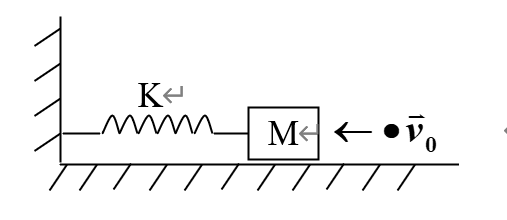
\includegraphics[width=0.15\textheight]{fig28}
                \caption{如图}\label{fig:28}
        \end{figure}
     \item 一质量为$m$的物体, 从质量为$M$的圆弧形槽顶端由静止滑下, 设圆弧形槽的半径为$R$, 张角为$\pi/2$,如图所示\ref{fig:26}, 如所有摩擦都可忽略,求:
    \begin{enumerate}
            
    \item[(1)] 物体刚离开槽底时,物体和槽的速度各是多少?
    \item[(2)] 在物体从A滑到B的过程中,物体对槽做的功为多少?
    \end{enumerate}
        \begin{figure}[ht]
            \centering
            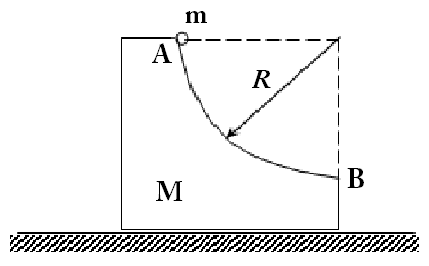
\includegraphics[width=0.15\textheight]{fig26}
                \caption{如图}\label{fig:26}
        \end{figure}
    \item 传送带$A$以 $v_0=2m\cdot s^{-1}$的速度把$m=20kg$的行李包送到坡道的上端, 行李包沿光滑的坡道下滑后装到$M=40kg$的小车上(如图\ref{fig:27}), 已知小车与传送带之间的高度差$h=0.6m$,
    行李包与车板间的摩擦系数$\mu =0.5$, 小车与地面的摩擦忽略不计, 取$g=10m\cdot s^{-2}$.求:
    \begin{enumerate}
        \item[(1)] 开始时行李包与车板间有相对滑动, 当行李对小车相对静止时车的速度.
        \item[(2)] 从行李包送上小车到它相对于小车为静止时, 所需的时间.	
    \end{enumerate}
    \begin{figure}[H]
        \centering
        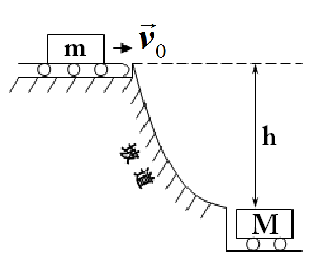
\includegraphics[width=0.15\textheight]{fig27}
            \caption{如图}\label{fig:27}
    \end{figure}
    
\end{enumerate}

\section{习题参考答案}
\subsection*{一、填空题}
\begin{enumerate}
    \item 如图所示 \ref{Fig:19} , 质量为$m$的子弹以水平速度$\vec{v_0}$射入静止的木块并陷入木块内, 
    设子弹入射过程中木块$M$不反弹, 则墙壁对木块的冲量$\vec{I}=\anl{$-m\vec{v_0}$}$ .
    \begin{note}
        \textcolor{red}{系统在子弹射入前总能量为$\vec{p_0}=m\vec{v_0}$, 子弹深入后因木块不反弹故系统总动量为0, $p=0$, 由质点系动量定理$\vec{I}=-m\vec{v_0}$}
    \end{note}
    \begin{figure}[H]
        \centering
        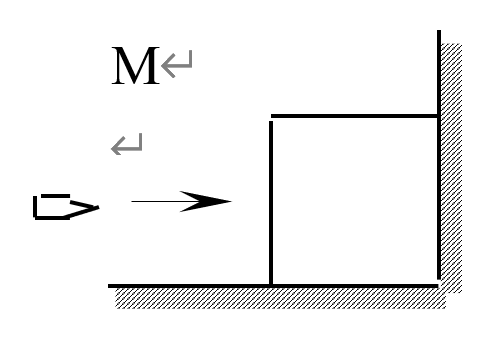
\includegraphics[width=0.15\textheight]{fig19}
            \caption{如图}\label{Fig:19}
    \end{figure}
    \item 一质量为 $m$ 的物体, 以初速$\vec{v_0}$从地面竖直上抛, 如忽略空气阻力, 则从抛出到刚要接触地面的过程中,物体动量增量的大小为\anl{$2mv_0$} .
    \item 一质量为$m$的物体作斜抛运动,初速率为$v_0$, 仰角为$\theta$. 如果忽略空气阻力, 物体从抛出点到最高点这一过程中所受合外力的冲量大小$I=\anl{$mv_0\mathrm{sin}\theta$}$.
    \item 有一质量为$M$的物体, 在光滑的水平面上沿直线滑行, 当它滑到某处速率为$v_0$时发生爆炸, 从主体上射出一质量为$m$的小块沿原方向水平飞行, 此时主体的速度为零, 则小块射出时对地的速率$v=\anl{$(M/m)v_0$}$.
    \item 一质量为$30 kg$的物体以$10m\cdot s^{-1}$的速率水平向东运动, 另一质量为$20 kg$的物体以$25 m\cdot s^{-1}$的速率水平向西运动. 两物体发生完全非弹性碰撞后, 它们的速度大小$v=\anl{$4 m\cdot s^{-1}$}$.
    \item 质量为 $M$ 的平板车, 以速度$\vec{v}$在光滑的水平面上滑行, 一质量为$m$的物体从$h$高处竖直落到车子里,两者一起运动时的速度大小为$V=\anl{$\frac{Mv}{M+m}$}$.
    \item 一颗质量为 $0.002kg$ , 速率为$700 m/s$的子弹, 打穿一块木板后,速率降到$400 m/s$, 则在此过程中受到的外力所做功$A=\anl{$-330 J$}$.
    \item 如图 \ref{Fig:20} , 有人用恒力$F$, 通过轻绳和轻滑轮, 将一木块从位置$A$拉到位置$B$, 设物体原来位置$AC=L$, 后来位置$BC=L/2$, 物体水平位移为$S$, 则在此过程中,人所作的功为$A=\anl{$FL_0/2$}$.
    \begin{figure}[H]
        \centering
        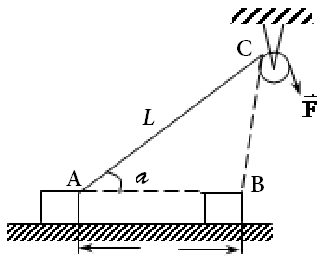
\includegraphics[width=0.15\textheight]{fig20}
            \caption{如图}\label{Fig:20}
    \end{figure}
    \item 某质点在力$ \vec{F}=(5+5x)\vec{i}$ (SI)的作用下沿$x$轴作直线运动, 在从$x=0$移动到$x=20m$的过程中, 力$\vec{F}$所做的功为\anl{$1100 J$} .
    \item 如图所示\ref{Fig:21} , 小球沿固定的光滑的$1/4$圆弧从$A$点由静止开始下滑, 圆弧半径为$R$, 则小球在$B$点处的法向加速度$a_n = \anl{2g}$; 切向加速度为 $a_t =\anl{0}$. 
    \begin{figure}[H]
        \centering
        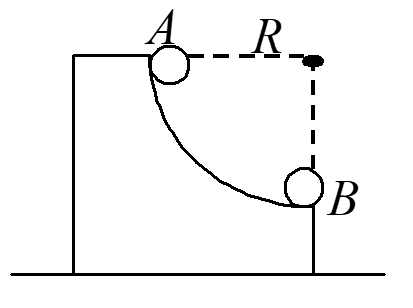
\includegraphics[width=0.15\textheight]{fig21}
            \caption{如图}\label{Fig:21}
    \end{figure}
    \item 人造地球卫星, 质量为$m$, 在地球表面上空2倍于地球半径$R$的高度沿圆轨道运行, 卫星的万有引力势能为\anl{$\frac{-GMm}{3R}$}. (用$m$、$R$、引力常数$G$和地球的质量$M$表示)
    \item 质量为$100kg$的货物, 平放在卡车底板上.卡车以$5m/s^2$的加速度启动, 货物与卡车底板无相对滑动. 则在开始的4秒钟内摩擦力对该货物作的功$A=\underline{2\times 10^4 J }$.
    \item 一个质量为$m=3kg$的质点, 在外力作用下, 运动方程为: $x=5+t^2$, $y=5t-t^2$, 则力在$t=0$到$t=2$秒内作的功为$A = \anl{-12 J}$.
\end{enumerate}
\subsection*{二、选择题}
\begin{enumerate}
    \item 一炮弹由于特殊原因在水平飞行过程中, 突然炸裂成两块, 其中一块作自由下落, 则另一块着地点(飞行过程中阻力不计):( A )   
    \twoch{比原来更远;}{比原来更近;}{仍和原来一样远;}{条件不足,不能判定.}
    \begin{note}
        \textcolor{red}{炸裂过程中, 水平方向动量守恒 $(m_1+m_2)v_0 = m_2v_2$}
    \end{note}  
    \item 质量为$0.02kg$的子弹, 以$400 m/s$的速率沿图示方向 \ref{Fig:22} 射入一原来静止的质量为$0.98kg$的摆球中, 摆线长度不可伸缩.子弹射入后开始与摆球一起运动的速率为( B )
    \fourch{$2m/s$}{$4m/s$}{$7m/s$}{$8m/s$} 
    \begin{figure}[H]
        \centering
        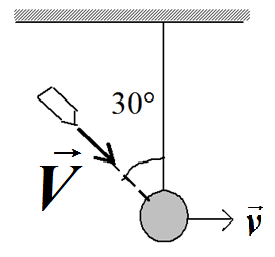
\includegraphics[width=0.15\textheight]{fig22}
            \caption{如图}\label{Fig:22}
    \end{figure}
    \begin{note}
        \textcolor{red}{子弹射入过程中, 水平方向动量守恒 $mv_0\mathrm{sin 30^\circ = (m+M)v}$}
    \end{note}
    \item 质量为$20 g$的子弹沿$x$轴正向以$500 m/s$的速率射入一木块后, 与木块一起仍沿$x$轴正向以$50 m/s$的速率前进, 在此过程中木块所受冲量的大小为( A )                                                        
    \twoch{$9 N\cdot s$}{$11 N\cdot s$}{$10 N\cdot s$}{$-10 N\cdot s$}
    \item 质量为$m$的质点, 以不变速率$v$沿水平光滑轨道垂直撞击墙面, 撞击后被反弹, 假设撞击为完全弹性碰撞, 并规定碰撞前质点运动方向为正方向,则质点作用于墙面的冲量为( B )
    \fourch{$mv$}{$2mv$}{$-mv$}{$-2mv$}
    \begin{note}
        \textcolor{red}{质点受墙面冲量为 $I=-mv-mv = -2mv$, 质点作用于墙面的冲量 $I^{'}=-I=2mv$}
    \end{note}
    \item 有两个完全相同的木块同时从同一高度自由落下, 在下落过程中有一水平方向飞来的子弹(其质量不可忽略不计)击中其中的一个木块, 并与木块一起下落, 则( B )  
   \twoch{两木块同时落地;}{被击中的木块后落地;}{被击中的木块先落地;}{无法判断}
   \begin{note}
       \textcolor{red}{水平方向动量守恒 $mv_x = (M+m)V_x^{'}$; 竖直方向动量守恒 $Mv_y = (M+m)V_y^{'}$; $\therefore v_y>V_y^{'}$}
   \end{note}
   \item  两辆小车$A$、$B$, 可在光滑平直轨道上运动. $A$以$2 m/s$的速率向右与静止的$B$对心碰撞, $A$和$B$的质量相同, 假定车$A$的初始速度方向为正方向,则碰撞为完全弹性碰撞和完全非弹性碰撞时车$A$的速度分别为( B )                         
   \twoch{$v_A=0 m/s$, $v_A=2 m/s$}{$v_A=0 m/s$, $v_A=1 m/s$}{$v_A=1 m/s$, $v_A=0 m/s$}{$v_A=2 m/s$, $v_A=1 m/s$}
    \item 一质量为$m$的质点, 自半径为$R$的光滑半球形碗口由静止下滑, 质点在碗内某处的速率为$v$, 则质点对该处的压力数值为( B )                
    \fourch{$\frac{mv^2}{R}$}{$\frac{3mv^2}{2R}$}{$\frac{2mv^2}{R}$}{$\frac{5mv^2}{2R}$}
    \item 质量为$m=0.5kg$的质点, 在Oxy坐标平面内运动, 其运动方程为$x=5t$, $y=0.5t^2$(SI), 从$t=2s$到$t=4s$这段时间内, 外力对质点作的功为( C )
    \fourch{$1.5 J$}{$4.5 J$}{$3 J$}{$-1.5 J$}
    \begin{note}
        看图, 懒得自己写了(其实自己写得不咋样):
    \end{note}
    \begin{figure}[H]
        \centering
        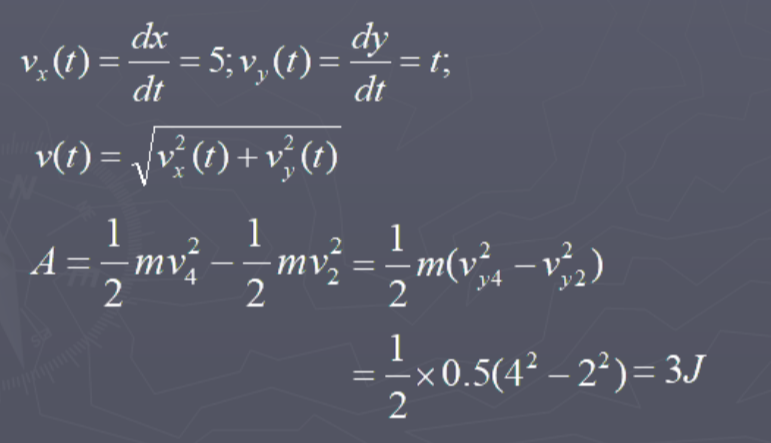
\includegraphics[width=0.25\textheight]{ans15}
    \end{figure}
    \item 如图 \ref{Fig:23} , 一质量为$m$的质点, 在半径为$R$的半球形容器中, 由静止开始自边缘上的$A$点滑下, 到达最低点$B$时, 它对容器的正压力为$N$. 则质点自$A$滑到$B$的过程中, 摩擦力对其作的功为( A )
    \twoch{$\frac{1}{2}R(N-3mg)$}{$\frac{1}{2}R(3mg-N)$}{$\frac{1}{2}R(N-mg)$}{$\frac{1}{2}R(N-2mg)$}
    \begin{figure}[H]
        \centering
        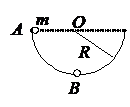
\includegraphics[width=0.15\textheight]{fig23}
            \caption{如图}\label{Fig:23}
    \end{figure}
    \item 光滑水平面上有一质量为$m=1kg$的物体, 在力$\vec{F} = (1+x)\vec{i}$  (SI) 作用下由静止开始运动, 当物体从$x_1$处运动到$x_2$处, 在此过程中物体的动能增量为( B )
    \twoch{$\left(x_1+\frac{x_1^2}{2}\right)-\left(x_2+\frac{x_2^2}{2}\right)$}{$\left(x_2+\frac{x_2^2}{2}\right)-\left(x_1+\frac{x_1^2}{2}\right)$}{$\left(x_1+\frac{x_1^2}{2}\right)$}{$\left(x_2+\frac{x_2^2}{2}\right)$}
    \begin{note}
        \textcolor{red}{ 根据动能定理 $\mathrm{d}E_k = \mathrm{d}A = F\mathrm{d}x = (1+x)\mathrm{d}x$\ \ \\
        $\therefore E_k = \displaystyle{\int_0^{E_k}\mathrm{d}E_k=\int_{x_1}^{x_2}\mathrm{d}x = \left(x_2+\frac{x_2^2}{2}\right)-\left(x_1+\frac{x_1^2}{2}\right)}$}
    \end{note}
    \item 在高台上分别沿$45^\circ$仰角方向和水平方向, 以同样速率投出两颗小石子, 忽略空气阻力, 则它们落地时速度( B )
    \twoch{大小不同,方向不同;}{大小相同,方向不同;}{大小相同,方向相同;}{大小不同,方向相同.}
    \item 在经典力学中,关于动能、功、势能与参考系的关系,下列说法正确的是( B )
    \onech{动能和势能与参考系的选取有关;}{动能和功与参考系的选取有关;}{势能和功与参考系的选取有关;}{动能、势能和功均与参考系选取无关.}
    \item 两辆小车$A$、$B$, 可在光滑平直轨道上运动. $A$以$3 m/s$的速率向右与静止的$B$碰撞, $A$和$B$的质量分别为$1kg$和$2kg$, 碰撞后$A$、$B$车的速度分别为$-1 m/s$和$2 m/s$, 则碰撞的性质为( A )    
    \twoch{完全弹性碰撞;}{完全非弹性碰撞 ;}{非完全弹性碰撞 ;}{无法判断 .}
    \item $A$、$B$二弹簧的劲度系数分别为$k_A$和$k_B$, 其质量均忽略不计. 今将二弹簧连接起来并竖直悬挂, 如图所示\ref{Fig:24} , 当系统静止时, 二弹簧的弹性势能$E_{PA}$与$E_{PB}$之比为( C )                                                 
    \twoch{$\frac{E_{PA}}{E_{PB}}=\frac{k_B}{k_A}$}{$\frac{E_{PA}}{E_{PB}}=\frac{k_A^2}{k_B^2}$}{$\frac{E_{PA}}{E_{PB}}=\frac{k_A}{k_B}$}{$\frac{E_{PA}}{E_{PB}}=\frac{k_B^2}{k_A^2}$}
    \begin{figure}[H]
        \centering
        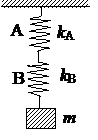
\includegraphics[width=0.15\textheight]{fig24}
            \caption{如图}\label{Fig:24}
    \end{figure}

    \item 质点的动能定理: 外力对质点所做的功, 等于质点动能的增量, 其中所描述的外力为( D )                                           
    \twoch{质点所受的任意一个外力;}{质点所受的保守力;}{质点所受的非保守力;}{质点所受的合外力.}
   
\end{enumerate}
\subsection*{三、计算题}
\begin{enumerate}
    \item 一个质量为$M$的四分之一圆弧形槽的大物体, 半径为$R$, 停在光滑的水平面上, 另一质量为$m$的物体, 自圆弧槽的顶端由静止下滑 (如图所示\ref{Fig:25}) .
    求当小物体$m$滑到弧底时, 大物体在水平面上移动的距离为多少?
    \begin{figure}[H]
        \centering
        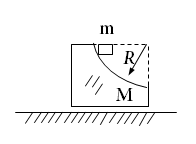
\includegraphics[width=0.15\textheight]{fig25}
            \caption{如图}\label{Fig:25}
    \end{figure}
    \begin{solution}
        看图: 
        \begin{figure}[H]
            \centering
            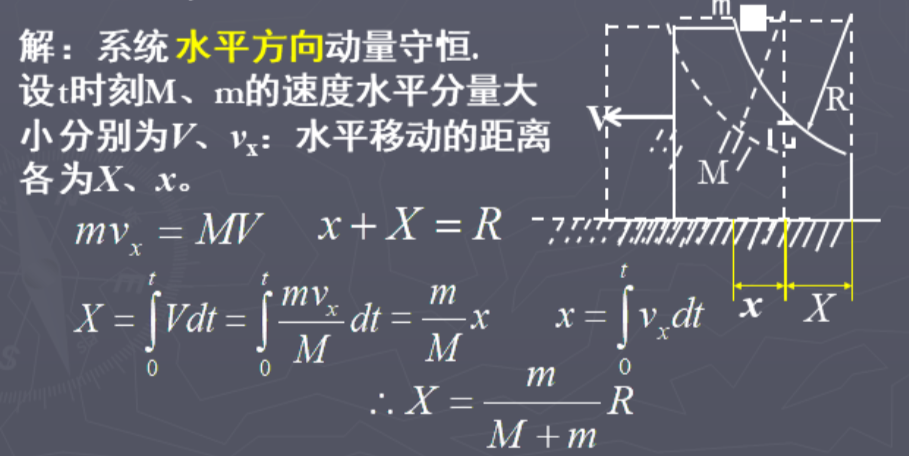
\includegraphics[width=0.48\textheight]{ans16}
        \end{figure}
    \end{solution}
    \item 一个质量为$M=10kg$的物体放在光滑水平面上, 并与一水平轻弹簧相连, 如图\ref{Fig:28}, 弹簧的劲度$K=1000N·m-1$, 今有一质量为$m=1kg$的小球, 
    以速度$V_0=4m\cdot s^{-1}$沿水平方向飞来, 并与物体M相撞后以$V1=2m\cdot s^{-1}$的速度弹回.试求:
    \begin{enumerate}
        \item[(1)] 碰撞之后, $M$的初速度是多少?
        \item[(2)] $M$起动后, 弹簧将被压缩,弹簧最大可缩短多少?
    \end{enumerate}
        \begin{figure}[H]
            \centering
            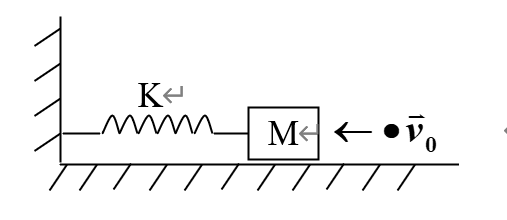
\includegraphics[width=0.15\textheight]{fig28}
                \caption{如图}\label{Fig:28}
        \end{figure}
        \begin{solution}
            \begin{enumerate}
                \item[(1)] 动能守恒: $mV_0=-mV_1 + MV$, $V=0.6 m/s$.
                \item[(2)] 机械能守恒: $\frac{1}{2}MV^2 = \frac{1}{2}Kx^2$, $x=0.06 m$
            \end{enumerate}
        \end{solution}
     \item 一质量为$m$的物体, 从质量为$M$的圆弧形槽顶端由静止滑下, 设圆弧形槽的半径为$R$, 张角为$\pi/2$,如图所示\ref{Fig:26}, 如所有摩擦都可忽略,求:
    \begin{enumerate}
            
    \item[(1)] 物体刚离开槽底时,物体和槽的速度各是多少?
    \item[(2)] 在物体从A滑到B的过程中,物体对槽做的功为多少?
    \end{enumerate}
        \begin{figure}[ht]
            \centering
            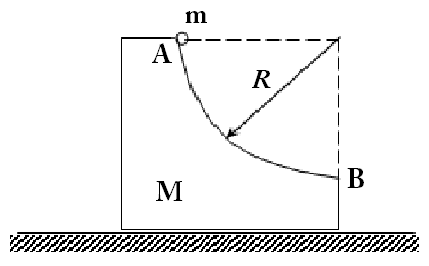
\includegraphics[width=0.15\textheight]{fig26}
                \caption{如图}\label{Fig:26}
        \end{figure}
        \begin{solution}
            看图: 
            \begin{figure}[H]
                \centering
                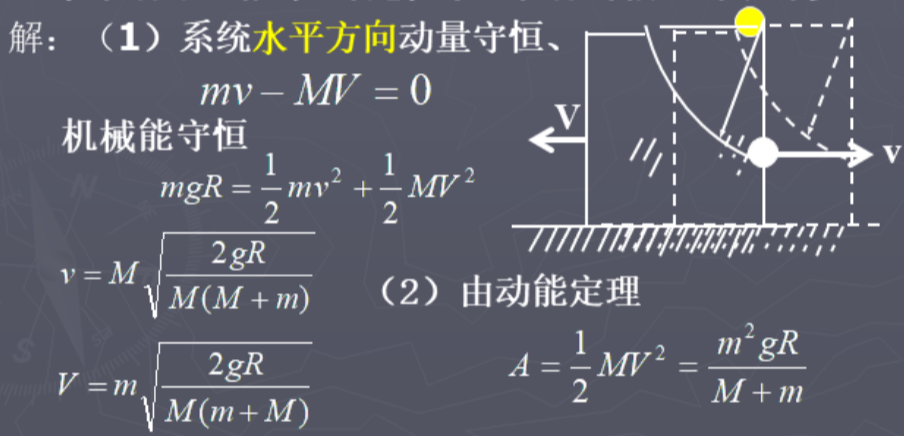
\includegraphics[width=0.48\textheight]{ans17}
            \end{figure}
        \end{solution}
    \item 传送带$A$以 $v_0=2m\cdot s^{-1}$的速度把$m=20kg$的行李包送到坡道的上端, 行李包沿光滑的坡道下滑后装到$M=40kg$的小车上(如图\ref{Fig:27}), 已知小车与传送带之间的高度差$h=0.6m$,
    行李包与车板间的摩擦系数$\mu =0.5$, 小车与地面的摩擦忽略不计, 取$g=10m\cdot s^{-2}$.求:
    \begin{enumerate}
        \item[(1)] 开始时行李包与车板间有相对滑动, 当行李对小车相对静止时车的速度.
        \item[(2)] 从行李包送上小车到它相对于小车为静止时, 所需的时间.	
    \end{enumerate}
    \begin{figure}[H]
        \centering
        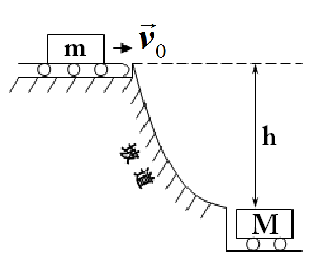
\includegraphics[width=0.15\textheight]{fig27}
            \caption{如图}\label{Fig:27}
    \end{figure}
    \begin{solution}
        看图: 
        \begin{figure}[H]
            \centering
            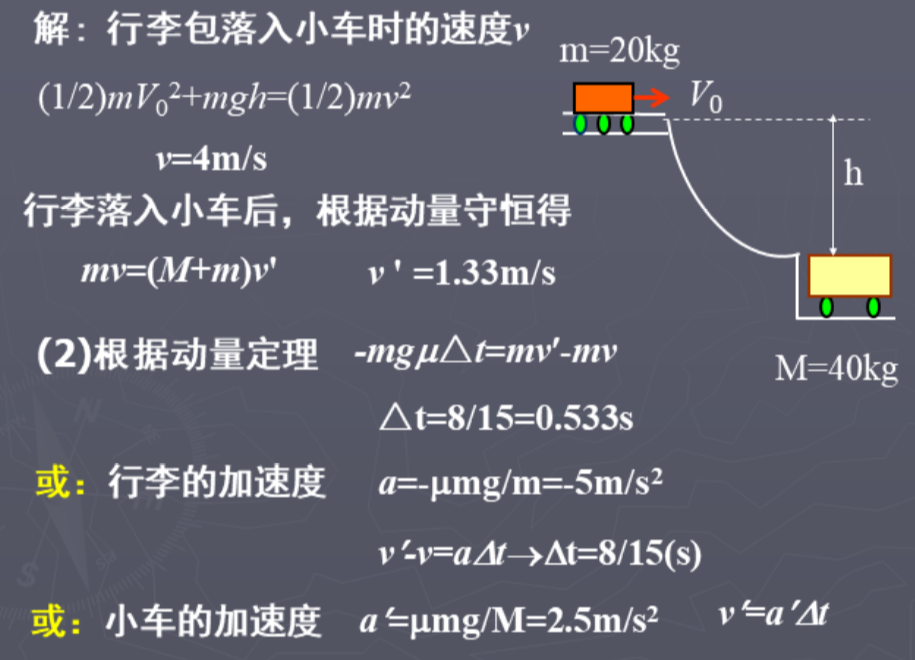
\includegraphics[width=0.48\textheight]{ans18}
        \end{figure}
    \end{solution}
    
\end{enumerate}